\documentclass[12pt]{article}
\usepackage[russian]{babel}
\usepackage{geometry}

%библиотеки для задания 2
\usepackage{graphicx}
\usepackage{caption}

\usepackage{enumitem}

%нестандартные математические обозначения
\usepackage{amssymb}
\usepackage{amsmath}

%различные цветовые модели
\usepackage[usenames]{color}
\usepackage[dvipsnames,table]{xcolor}
\usepackage{colortbl}

\usepackage{listings}
\usepackage{listingsutf8}
\usepackage[T2A]{fontenc}
\newcommand{\listingsttfamily}{\usefont{T2A}{PTMono-TLF}{m}{n}}

\lstset{
	language=C,                % choose the language of the code
	numbers=left,                   % where to put the line-numbers
	stepnumber=1,                   % the step between two line-numbers.        
	numbersep=5pt,                  % how far the line-numbers are from the code
	backgroundcolor=\color{black},  % choose the background color. You must add \usepackage{color}
	commentstyle=\color{Gray},
	basicstyle=\listingsttfamily\color{Gray},
	keywordstyle=\color{BurntOrange},
	stringstyle=\color{YellowGreen},
	showspaces=false,               % show spaces adding particular underscores
	showstringspaces=false,         % underline spaces within strings
	showtabs=false,                 % show tabs within strings adding particular underscores
	tabsize=4,                      % sets default tabsize to 2 spaces
	captionpos=b,                   % sets the caption-position to bottom
	breaklines=true,                % sets automatic line breaking
	breakatwhitespace=true,         % sets if automatic breaks should only happen at whitespace
	title=\lstname, 
	inputencoding=utf8,                % show the filename of files included with \lstinputlisting;
	extendedchars=\true,
	keepspaces=true
}

%параметры документа
\geometry{top=2cm, bottom=2cm, left=1cm, right=1cm}
\textheight=24cm
\textwidth=18cm
\flushbottom 

\oddsidemargin=0pt 
\topmargin=-1.5cm 
\parskip=0pt
\parindent=24pt 

\tolerance=2000 

\begin{document}
	\begin{center}
		{\parskip=1cm
			МИНИСТЕРСТВО НАУКИ И ВЫСШЕГО ОБРАЗОВАНИЯ РОССИЙСКОЙ ФЕДЕРАЦИИ
			
			ФЕДЕРАЛЬНОЕ ГОСУДАРСТВЕННОЕ БЮДЖЕТНОЕ ОБРАЗОВАТЕЛЬНОЕ УЧРЕЖДЕНИЕ ВЫСШЕГО ОБРАЗОВАНИЯ
			
			{\bf«БЕЛГОРОДСКИЙ ГОСУДАРСТВЕННЫЙ ТЕХНОЛОГИЧЕСКИЙ УНИВЕРСИТЕТ им. В. Г. Шухова»\\(БГТУ им. В. Г. Шухова)}
			
			
			\begin{figure}[bh]
			\noindent\centering{
				
\includegraphics[width=100mm]{images/start_logo.png}
				\captionsetup{labelformat=empty}
			}
			\end{figure}
			Кафедра программного обеспечения вычислительной техники и автоматизированных систем
		}
		{\parskip=0.25cm
			{\Large 
				{\bf Лабораторная работа №4}
			
				по дисциплине: <<Алгоритмы и структуры данных>>
			
				по теме: {\bf <<Сравнительный анализ методов поиска (C)>>}
			}
		}
	\end{center}
	\begin{flushright}
		{\parskip=3cm Выполнил/a: ст. группы ПВ-231}
		
		Чупахина София Александровна
		
		Проверил:
		
		Акиньшин Даниил Иванович
	\end{flushright}
	\begin{center}
		{\parskip=3cm Белгород, 2024}
	\end{center}
	\newpage
	
	{\bf Цель работы:} изучение алгоритмов поиска элемента в массиве и закрепление навыков в проведении сравнительного анализа алгоритмов.
	
	{\bf Задания:}
	
	\setlist[1]{noitemsep} % sets the itemsep and parsep for all level two lists to 0
	
	\begin{enumerate}
	
	\item Изучить алгоритмы поиска:
	
		\begin{enumerate}
	
			\item в неупорядоченном массиве:
			
			\begin{enumerate}
	
				\item линейный;
	
				\item быстрый линейный;
			
			\end{enumerate}
	
	
			\item в упорядоченном массиве:
			
			\begin{enumerate}
	
				\item быстрый линейный;
	
				\item бинарный;
	
				\item блочный.
				
			\end{enumerate}
	
		\end{enumerate}
	
	\item Разработать и программно реализовать средство для проведения экспериментов по определению временных характеристик алгоритмов поиска.
	
	\item Провести эксперименты по определению  временных характеристик алгоритмов поиска. Результаты экспериментов представить в виде таблиц 1 и 2. Клетки таблицы 1 содержат максимальное количество операций сравнения при выполнении  алгоритма поиска, а клетки таблицы 2 — среднее число операций сравнения.
	
	\item Построить графики зависимости количества операций сравнения от количества элементов в массиве.
	
	\item Определить аналитическое выражение функции зависимости количества операций сравнения от количества элементов в массиве.
	
	\item Определить порядок функций временной сложности алгоритмов поиска.
	
	
	\end{enumerate}
	
	\tableofcontents
	\newpage
	
	\section{Задание 1:}
	\label{task_1}
	Кратко опишем данные алгоритмы поиска:
	
	\subsection{На неупорядоченном массиве:}
	\label{task_1_1}
	\subsubsection{Задание 1.1.1:}
	\label{task_1_1_1}
	
	Линейный поиск --- самая простая разновидность поиска. Его можно применять как в упорядоченном, так и в неупорядоченном массиве. В начале функции, реализующей этот алгоритм, создается переменная текущего индекса, начальное значение которой равно 0. Затем запускается цикл, с каждой итерацией которого текущий индекс увеличивается на 1; цикл продолжает выполняться до тех пор, пока элемент под этим индексом не станет равен искомому, либо же до тех пор, пока индекс не станет равен размеру массива. После завершения цикла выполняется проверка, равен ли текущий индекс размеру массива. Если да, то это значит, что за проход по массиву не был найдет искомый элемент: в таком случае функция возвращает -1, иначе возвращается текущий индекс. 
	
	\lstinputlisting[firstline=4, lastline=10]{../АСД 4 си/search_algorithms.c} 
	
	{\parskip=0.15cm
	
	\subsubsection{Задание 1.1.2:}
	\label{task_1_1_2}
	
	Линейный поиск можно модифицировать следующим образом. В его стандартной реализации условие цикла состоит из двух частей: проверки на то, равен ли элемент под текущим индексом искомому, и на то, сравнялся ли текущий индекс с длиной массива. Избавиться от второй проверки можно, если в конец массива (после всех элементов, на позицию с индексом, равным его размеру) добавить элемент, равный искомому. (Тогда для нормальной работы программы необходимо запомнить элемент, находящийся на этой позиции, как бы за пределами массива, потом заменить его на искомый, а после прохода по массиву вернуть ему изначальное значение). Тогда, после установки стартового значения текущего индекса в 0, в условии цикла достаточно проверять, равен ли искомому элемент под текущим индексом; при достижении конца оригинального массива равенство будет верным.  Тогда после завершения цикла выполняется такая же проверка, как и в стандартном алгоритме линейного поиска. Если текущий индекс равен размеру массива, то в самом массиве искомый элемент отсутствует, и функция возвращает -1, иначе --- текущий индекс.  
	
	\lstinputlisting[firstline=12, lastline=21]{../АСД 4 си/search_algorithms.c} 
	
	\subsection{На упорядоченном массиве:}
	\label{task_1_2}
	\subsubsection{Задание 1.2.1:}
	\label{task_1_2_1}
	
	При использовании алгоритмов линейного либо быстрого линейного поиска поиске в неупорядоченном массиве, мы должны перебирать элементы под всеми возможными индексами, пока не найдем искомый элемент либо не достигнем конца массива. Однако если известно, что массив упорядочен, то область поиска можно уменьшить: как только находится элемент, больший искомого, можно сделать вывод, что и среди дальнейших элементов массива искомого не будет. Модифицируем алгоритм быстрого линейного поиска так, чтобы (после установки значения текущего индекса в 0) цикл продолжался до тех пор, пока элемент под текущим индексом меньше искомого (а не пока он не равен ему). В таком случае после завершения цикла необходимо выполнить две проверки: равен ли элемент под текущим индексом искомому и равен ли текущий индекс размеру массива. Выполнение хотя бы одного из этих условий означает, что в массиве нет искомого элемента: если выполнилось первое, то был встречен элемент больше искомого, если выполнилось второе, то был достигнут конец массива, отмеченный дополнительным искомым элементом. В таком случае возвращается значение -1, иначе возвращается текущий индекс.
	
	\lstinputlisting[firstline=23, lastline=32]{../АСД 4 си/search_algorithms.c} 
	
	\subsubsection{Задание 1.2.2:}
	\label{task_1_2_2}
	
	Бинарный поиск, предназначенный для применения в упорядоченных массивах, тоже использует идею ограничения области поиска. В начале алгоритма устанавливаются индексы левой и правой границ поиска, равные соответственно 0 и размеру массива, уменьшенному на 1. Переменная, хранящая индекс искомого элемента, инициализируется со значением -1 (по умолчанию элемент считается не найденным). Затем запускается цикл, в котором для текущих индексов границ находится индекс элемента, стоящего посередине. Если элемент под этим индексом равен искомому, то значение переменной индекса искомого элемента приравнивается к <<серединному>> индексу, и выполнение цикла досрочно завершается. Иначе сдвигается одна из границ области поиска: если элемент под серединным индексом меньше искомого, то новое значение индекса левой границы --- увеличенный на 1 серединный индекс, иначе новое значение правой границы --- уменьшенный на 1 серединный индекс. Выполнение цикла прекращается, когда область писка перестает включать в себя хотя бы один элемент, то есть индекс левой границы становится больше индекса правой. Тогда возвращается переменная, хранящая индекс искомого значения; она равна -1, если цикл был завершен из-за вырождения области поиска, и индексу искомого элемента, если он был найден и, соответственно, цикл завершился досрочно.
	
	\lstinputlisting[firstline=34, lastline=49]{../АСД 4 си/search_algorithms.c} 
	
	\subsubsection{Задание 1.2.3:}
	\label{task_1_2_3}
	
	Блочный поиск базируется на следующей идее. При быстром линейном поиске в упорядоченном массиве мы перебираем элементы один за другим, опираясь на тот факт, что если был встречен элемент больше искомого, то его нет и среди следующих. Но также справедливо то, что если некоторый элемент меньше искомого, то среди предыдущих элементов его также нет. Опираясь на этот факт, мы могли бы перебирать элементы массива с некоторым шагом, разделяя его на блоки и начиная линейный поиск со <<сплошным>> перебором только в том блоке, последний элемент которого больше искомого. Но как найти оптимальный размер блока? В худшем случае, когда искомый элемент находится в конце массива (или не входит в массив вовсе, при этом его значение больше значения максимального элемента массива), при поиске придется дойти до последнего блока и осуществить линейный поиск в этом блоке. При размере массива N и размере блока n количество операций для перебора всех блоков будет пропорционально $\frac{N}{n}$, а количество операций для перебора всех значений блока будет пропорционально $n$. Общее количество операций будет пропорционально $\frac{N}{n} + n$, и чтобы найти значение $n$, при котором это выражение будет минимальным, необходимой найти его производную и приравнять ее к 0. $\frac{d(\frac{N}{n} + n)}{dn}$ = $-\frac{N}{n^2} + 1$, соответственно, $\frac{N}{n^2}$ = $1$, $n^2$ = $\frac{N}{1}$ = $N$ и $n$ = $\sqrt{N}$.
	
	Таким образом, алгоритм будет иметь следующую структуру. Значение шага, с которым будет совершаться проход, инициализируется как целая часть корня от размера массива, а текущий индекс устанавливается в 0. Затем, пока текущий индекс меньше размера массива, уменьшенного на величину шага (то есть пока блоки имеют нормальный, максимальный размер), в теле цикла сравниваются последний элемент блока (элемент под индексом, большим текущего на размер блока) и искомый элемент. Если искомый элемент меньше последнего элемента блока, то c помощью быстрого линейного поиска для упорядоченного массива находится <<относительный>> индекс искомого элемента, который прибавляется к текущему, и цикл прерывается. Иначе, то есть если нужный блок не был найден, к текущему индексу просто прибавляется размер шага. После завершения цикла похожая последовательность действий повторяется для последнего, <<нецелого>> блока, если последний элемент этого блока (то есть этого массива) не меньше искомого, если индекс искомого элемента все еще не найден и если текущий индекс находится за пределами последнего целого блока. Единственное, что меняется --- размер подмассива, в котором выполняется линейный поиск (в случае, если нецелого блока на самом деле нет, будет выполнен линейный поиск в пустом массиве). После проверки этого последнего блока возвращается -1, если индекс искомого элемента так и не был найден, то есть под текущим индексом не находится искомый элемент, иначе возвращается текущий индекс.
	
	\lstinputlisting[firstline=53, lastline=67]{../АСД 4 си/search_algorithms.c} 
	
	\section{Задание 2:}
	\label{task_2}
	Проведем эксперименты по вычислению временных характеристик алгоритмов поиска способом, похожим на тот, что мы использовали ранее (в лабораторной работе 3). 
	
	Для каждой функции поиска в отдельном файле создадим ее копию, которая, помимо возвращения индекса заданного элемента, изменяет значение переменной типа int по адресу compares, увеличивая его на количество сравнений, выполненных данной функцией поиска. Счетчик сравнений возрастает: 1) внутри каждого цикла while, 2) после выполнения каждого цикла, потому что проверка условия выполнялась и тогда, когда условие продолжения вернуло значение «ложь», тело цикла не было выполнено и счетчик сравнений не был увеличен, 3) перед каждой условной конструкцией. В каждом из этих случаев учитывается, из скольких частей состоит условие продолжения цикла или выполнения условной конструкции. Если функция использует вспомогательный алгоритм, то при вызове этого алгоритма ему в качестве адреса счетчика передается тот же адрес, и выполненные основной и вспомогательной функцией сравнения таким образом складываются --- поэтому нельзя устанавливать счетчик в ноль в теле функции. 
	
	В дополнение к функциям сортировки, объявим отдельные функции генерации неупорядоченного и упорядоченного массивов заданного размера, причем элементы неупорядоченного массива не повторяются. 
	
	И наконец, объявим две функции, выводящие строки таблицы максимального и среднего числа сравнений. Каждая из них принимает указатель на массив функций поиска, длину этого массива и функцию генерации массива, в котором будет производиться поиск. В теле цикла for перебираются функции поиска --- элементы соответствующего массива, и для каждой функции перебираются длины массива целых чисел, от 50 до 450 с шагом 50. Создается массив целых чисел в соответствии с переданной функцией генерации (упорядоченный или неупорядоченный), переменная для максимального либо суммарного количества сравнений, и затем запускается третий цикл, в котором перебираются все элементы массива целых чисел и осуществляется поиск каждого из них, при этом модифицируется переменная максимального или суммарного количества сравнений. В конце осуществляется дополнительный поиск числа, которого нет в массиве, для полноты картины, и после этого переменная максимального либо суммарного, разделенного на количество поисков, количества сравнений выводится на экран, сразу с разделителем, чтобы количество сравнений для следующего массива, с измененным размером, не сливалось с текущим значением. После достижения максимальной длины массива, при переходе к следующей функции, производится перенос строки.
	
	Объявив в теле функции main два массива функций поиска, и применив указанные функции по два раза (максимальное количество сравнений для поиска в неупорядоченном массиве, оно же для поиска в упорядоченном массиве, среднее количество сравнений для поиска в неупорядоченном массиве, оно же в упорядоченном массиве), выведем на экран требуемые данные.
	
	\lstinputlisting{../АСД 4 си/compares_testing.c} 
	
	\section{Задание 3:}
	\label{task_3}
	
	Теперь для получения таблиц с как максимальным, так и средним количеством сравнений для алгоритмов поиска на неупорядоченных и упорядоченных массивах с длинами от 50 до 450 с шагом 50, достаточно запустить программу и перенести результаты из консоли в таблицу.
	
	\begin{figure}[h]
		\noindent\centering{
			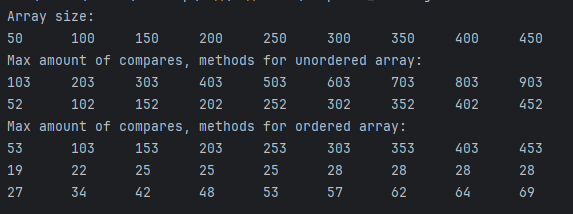
\includegraphics[width=160mm]{images/max_console.png}
			\caption{Данные для таблицы, отображающей максимальное количество сравнений для разных алгоритмов поиска, в консоли}
		}
	\end{figure}
	\begin{figure}[h]
		\noindent\centering{
			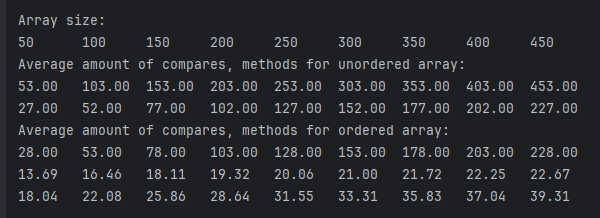
\includegraphics[width=160mm]{images/average_console.png}
			\caption{Данные для таблицы, отображающей среднее количество сравнений для разных алгоритмов поиска, в консоли}
		}
	\end{figure}
	
	\newpage
	
	\begin{figure}[h]
		\noindent\centering{
			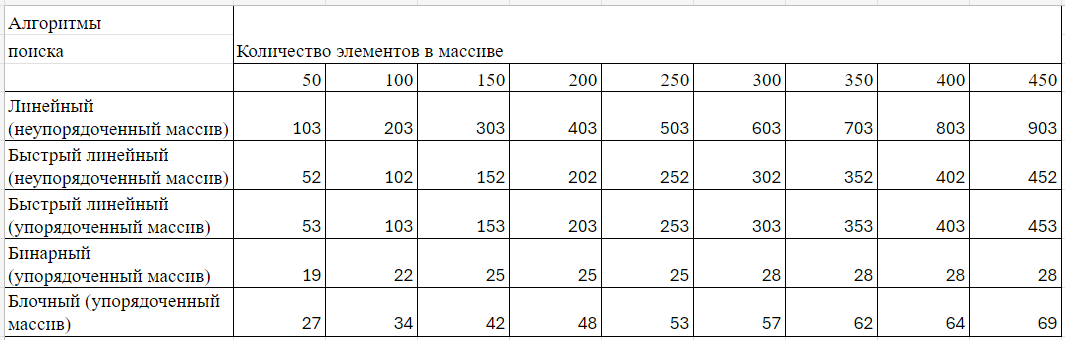
\includegraphics[width=170mm]{images/max_table.png}
			\caption{Таблица, отображающая максимальное количество сравнений для разных алгоритмов поиска}
		}
	\end{figure}
	\begin{figure}[h]
		\noindent\centering{
			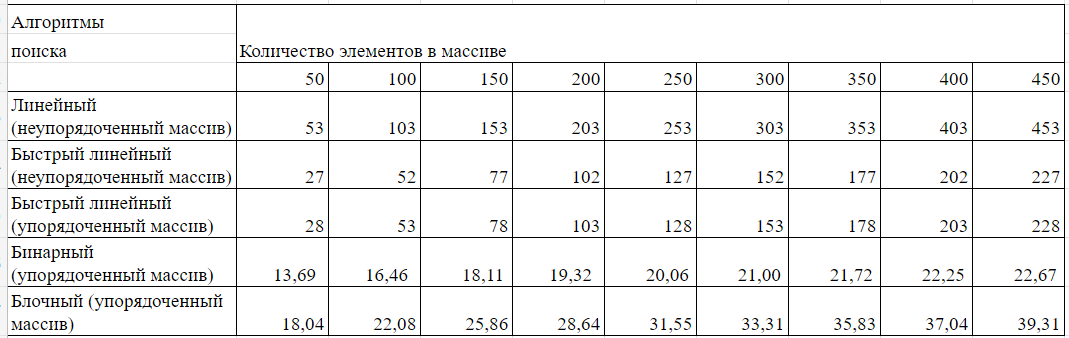
\includegraphics[width=170mm]{images/average_table.png}
			\caption{Таблица, отображающая среднее количество сравнений для разных алгоритмов поиска}
		}
	\end{figure}


	
	\section{Задание 4:}
	\label{task_4}
	
	По данным составленных таблиц легко построить график с помощью встроенных средств Excel. Стоит заметить, что и максимальные, и средние значения количества сравнений для быстрого линейного поиска в неупорядоченных и упорядоченных массивах очень близки, поэтому график для быстрого линейного поиска в неупорядоченных массивах едва различим.
	
	\newpage
	
	\begin{figure}[h]
		\noindent\centering{
			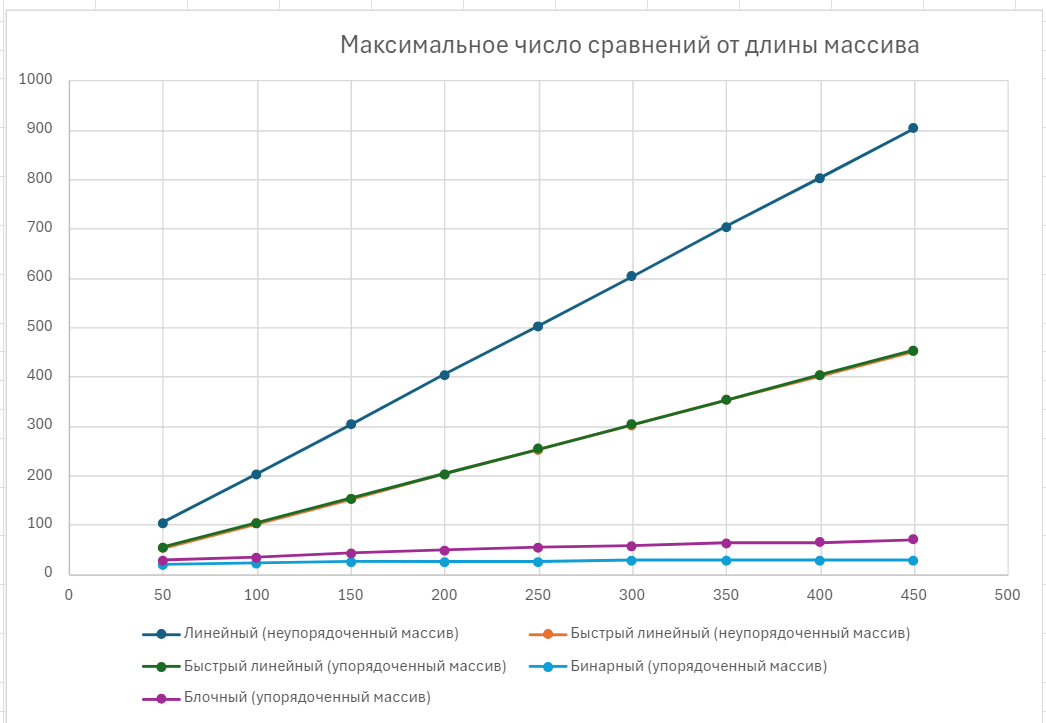
\includegraphics[width=150mm]{images/max_graph.png}
			\caption{График зависимости максимального количества сравнений для разных алгоритмов поиска от длины массива, в котором производится поиск}
		}
	\end{figure}
	
	\begin{figure}[h]
		\noindent\centering{
			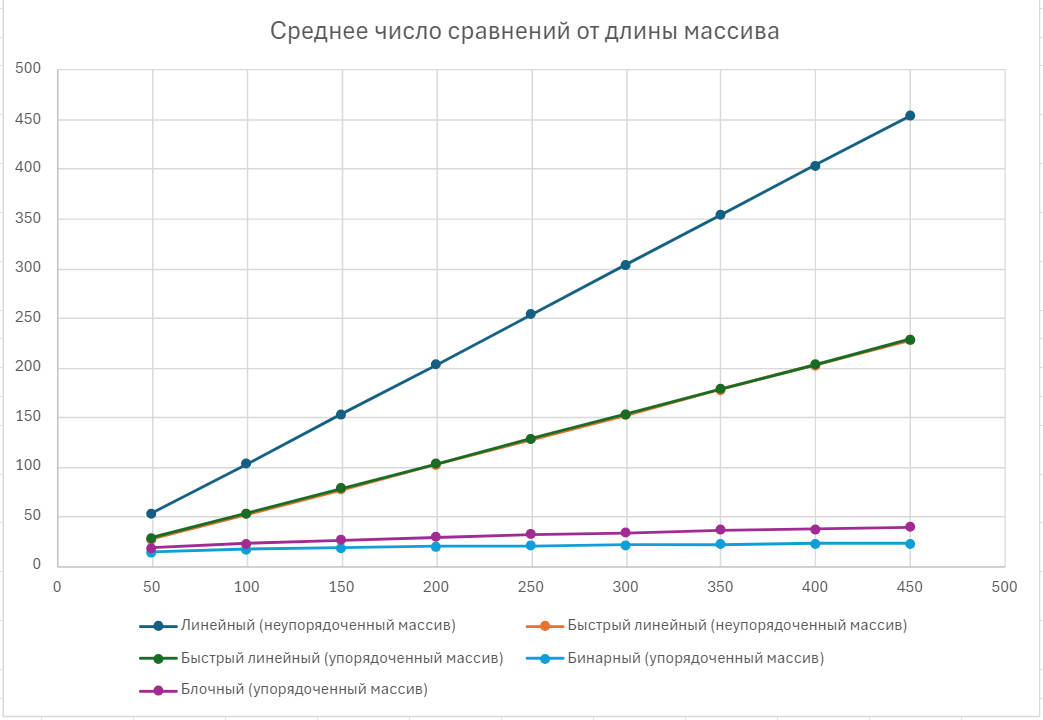
\includegraphics[width=150mm]{images/average_graph.png}
			\caption{График зависимости среднего количества сравнений для разных алгоритмов поиска от длины массива, в котором производится поиск}
		}
	\end{figure}
	\newpage
	
	
	\section{Задание 5:}
	\label{task_5}
	
	Примем длину рассматриваемого массива за n, и найдем аналитические выражения для максимального и среднего числа сравнений ри применении того или иного алгоритма поиска.
	
	Как мы уже говорили в задании 1.1.1, в начале алгоритма линейного поиска текущий индекс устанавливается в 0, и затем циклически увеличивается на 1, до тех пор, пока элемент под этим индексом не станет равен искомому либо пока индекс не выйдет за пределы массива. В худшем случае, когда искомого элемента нет в массиве вообще, будет выполнено n итераций цикла (сравнение каждого элемента массива с искомым), при выполнении каждой из которых производится 2 сравнения (проверка на выход за пределы массива и проверка на равенство текущего элемента искомому). Будем считать, что при выходе из цикла также производится 2 сравнения на те же условия (но в этот раз они возвращают ложь). Наконец, одно сравнение производится в конце алгоритма, и оно отвечает за проверку, равен ли текущий индекс размер массива. Суммарное количество сравнений в худшем случае составит $2\times(n+1) + 1$ = $2n + 2 + 1$ = $2n + 3$. 
	
	В лучшем же случае, когда искомый элемент --- первый в массиве, будет выполнено 2 сравнения для того, чтобы оборвать цикл на <<нулевой>> итерации, и 1 для стандартной проверки на то, выходит ли текущий индекс за пределы массива. Таким образом, в лучшем случае количество сравнений равно 3. Если же искомый элемент в массиве второй, то будет выполнено 2 сравнения на первую итерацию цикла (и увеличение на 1 текущего индекса), 2 на выход из цикла и 1 на проверку в конце, итого 5 сравнений. С увеличением индекса, под которым входит искомый элемент в массив, количество сравнений будет увеличиваться на 2. Среднее количество сравнений можно найти как сумму сравнений для всех возможных вариантов, от лучшего к худшему, на их количество $(n+1)$, а эту сумму --- как сумму арифметической прогрессии с разностью 2: $\frac{2\times3 + 2 \times(n+1-1)}{2}\times(n+1)$ = $\frac{2\times3 + 2 \times n}{2}\times(n+1)$. Итого количество сравнений будет равно $\frac{\frac{2\times3 + 2 \times n}{2}\times(n+1)}{n+1}$ = $\frac{2\times3 + 2 \times n}{2}$ = $3 + n$.
	
	Похожую логику можно применить при рассмотрении быстрого линейного поиска в неупорядоченном массиве. В худшем случае, когда искомого элемента нет в массиве вообще, будет выполнено n итераций цикла (сравнение каждого элемента массива с искомым), но при выполнении каждой производится 1 сравнение (только проверка на равенство текущего элемента искомому). Дополнительное сравнение для проверки того же условия производится при выходе из цикла, и одно сравнение производится в конце алгоритма. Суммарное количество сравнений в худшем случае составит $n+1 + 1$ = $n + 2$.
	
	Для нахождения среднего количества сравнений используем ту же формулу, включающую в себя сумму арифметической прогрессии, но с первым членом 1 и разностью 1: $\frac{2\times2 + (n+1-1)}{2}\times(n+1)$ = $\frac{2\times2 + n}{2}\times(n+1)$. Итого количество сравнений будет равно $\frac{\frac{2\times2 + n}{2}\times(n+1)}{n+1}$ = $\frac{2\times2 + n}{2}$ = $2 + \frac{n}{2}$.
	
	Ситуация для быстрого линейного поиска в упорядоченном массиве будет точно такой же, за исключением того, что в конце алгоритма выполняется 2 операции сравнения --- проверка на равенство элемента под текущим индексом искомому и проверка на выход из границ массива. В остальном все неизменно. В худшем случае, когда искомого элемента нет в массиве вообще и при этом этот элемент больше максимального элемента массива, будет выполнено n итераций цикла (сравнение каждого элемента массива с искомым), при выполнении каждой производится 1 сравнение (только проверка на равенство текущего элемента искомому). Дополнительное сравнение для проверки того же условия производится при выходе из цикла. Количество сравнений в худшем случае составит $n+1 + 2$ = $n + 3$, среднее же будет равно $3 + \frac{n}{2}$. Разница с быстрым линейным поиском в неупорядоченном массиве в количестве выполняемых операций будет заметна только в случае поиска элемента, не входящего в массив, но меньшего максимального: для неупорядоченного массива это будет худшим случаем, для упорядоченного количество операций будет зависеть от того, между элементами с какими индексами мог бы располагаться искомый. Но в нашей схеме подсчета среднего числа сравнений такие случаи не рассматриваются.
	
	Для бинарного поиска худшим случаем также будет отсутствие в массиве искомого элемента (неважно при этом, больше ли он максимального). В таком случае область поиска будет уменьшаться вдвое до тех пор, пока ее длина не окажется равной 0, и на каждую итерацию цикла, уменьшающего эту область, будет приходиться по 3 операции сравнения (проверка условия цикла, проверка элемента под серединным индексом на равенство искомому, которая всегда будет возвращать ложь, и проверка на то, больше или меньше серединный элемент искомого). Максимально возможное количество итераций при такой стратегии, когда область уменьшается вдвое, при этом в нее не включен серединный элемент, будет равно $\lceil \log_2{(n+1)}\rceil$. Еще одно сравнение будет совершено при проверке условия цикла на выходе из него, и количество сравнений в худшем случае, то есть максимально возможное, будет равно $3\times\lceil \log_2{(n+1)}\rceil + 1$.

	Далее рассмотрим лучший случай: когда искомый элемент будет являться серединным уже на первой итерации. В таком случае количество сравнений составит 2 (проверка условия цикла и проверка на равенство искомому с досрочным выходом). Элемент, для которого это возможно, в массиве только 1. Если же элемент равен серединному на второй итерации, то количество сравнений составит 3+2 = 5 (3 на итерацию с уменьшением области и 2 на итерацию, в которой индекс найден), и всего таких элементов существует уже 2 --- по одному на каждую половину массива после первой итерации. Если элемент равен серединному на третьей итерации, то количество сравнений составит 3+3+2 = 7, а всего элементов будет 4. Итого сумма сравнений для поиска всех возможных элементов составит:
	$$\sum_{0}^{\lfloor \log_2{(n+1)} \rfloor - 1}{((2+3\times i)\times2^i)} + (2+3\times \lfloor \log_2{(n+1)} \rfloor)\times (n - 2^{\lfloor \log_2{(n+1)} \rfloor} + 1)$$
	Прибавив к этому числу обозначенный нами худший случай и разделив сумму на $n+1$, получим аналитическое выражение для среднего количества сравнений:
	$$\frac{\sum_{0}^{\lfloor \log_2{(n+1)} \rfloor - 1}{((2+3\times i)\times2^i)} + (2+3\times \lfloor \log_2{(n+1)} \rfloor)\times (n - 2^{\lfloor \log_2{(n+1)} \rfloor} + 1) + 3\times\lceil \log_2{(n+1)}\rceil + 1}{n+1}$$
	
	Наконец, перейдем к блочному поиску. Для него рассмотрим только, когда блоки являются целыми, то есть длина массива делится на размер блока нацело. В отличие от остальных алгоритмов поиска, здесь худшим случаем будет являться не тот, когда нужного элемента нет в массиве вообще, а тот, когда нужный элемент --- последний в последнем блоке, причем размер последнего блока максимален. Тогда в случае, если имеется нецелый блок в конце, на перебор всех целых блоков уйдет $\frac{n}{\lfloor\sqrt{n}\rfloor}$ итераций, каждая из которых требует 2 сравнения (условие цикла и сравнение искомого элемента с конечным элементом блока), плюс 1 сравнение для выхода из цикла. На последней итерации будет выполнен быстрый линейный поиск в упорядоченном массиве длиной $\lfloor\sqrt{n}\rfloor$, что прибавит к счетчику $\lfloor\sqrt{n}\rfloor + 3$ сравнения (см. аналитическое выражение худшего случая для этого алгоритма поиска). Затем будет выполнено 3 сравнения на проверку наличия нецелого блока (они вернут ложь). Итого в худшем случае будет выполнено $2\times\frac{n}{\lfloor\sqrt{n}\rfloor} + 1 + \lfloor\sqrt{n}\rfloor + 3$ = $2\times\frac{n}{\lfloor\sqrt{n}\rfloor} + \lfloor\sqrt{n}\rfloor + 4$ операции сравнения.
	
	Рассмотрим теперь абстрактный средний случай. Чтобы найти суммарное количество сравнений для всех возможных случаев, разделим эти случаи на группы: элемент встречается в первом, втором, третьем блоке и так далее. Для искомых элементов в первом блоке сумма операций сравнения в ходе быстрого линейного поиска может быть вычислена как арифметическая прогрессия с первым членом 3, последним членом $2\times\lfloor\sqrt{n}\rfloor + 1$ и количеством элементов $\lfloor\sqrt{n}\rfloor$: $\frac{3 + 2\times\lfloor\sqrt{n}\rfloor + 1}{2} \times \lfloor\sqrt{n}\rfloor$ = $(\frac{\lfloor\sqrt{n}\rfloor}{2} + 2) \times \lfloor\sqrt{n}\rfloor$. При этом на каждый поиск в первом блоке придется 2 операции сравнения в первой итерации и 4 на финальные проверки. Итого количество операций сравнения в первом блоке составит $(\frac{\lfloor\sqrt{n}\rfloor}{2} + 2 + 2 + 4) \times \lfloor\sqrt{n}\rfloor$ = $(\frac{\lfloor\sqrt{n}\rfloor}{2} + 8) \times \lfloor\sqrt{n}\rfloor$. При поиске во втором блоке в ходе линейного поиска будет совершено столько же операций, при этом на каждый поиск потребуется 4 операции сравнения на 2 итерации цикла, 4 на финальную проверку. Итого количество сравнений о втором блоке = $(\frac{\lfloor\sqrt{n}\rfloor}{2} + 2 + 4 + 4) \times \lfloor\sqrt{n}\rfloor$ = $(\frac{\lfloor\sqrt{n}\rfloor}{2} + 10) \times \lfloor\sqrt{n}\rfloor$. Всего блоков $\frac{n}{\lfloor\sqrt{n}\rfloor}$, и количество сравнений в них всех можно посчитать как арифметическую прогрессию с первым членом $(\frac{\lfloor\sqrt{n}\rfloor}{2} + 8) \times \lfloor\sqrt{n}\rfloor$ и шагом $2\times\lfloor\sqrt{n}\rfloor$:
	
	$$\frac{2\times(\frac{\lfloor\sqrt{n}\rfloor}{2} + 8) \times \lfloor\sqrt{n}\rfloor + 2\times\lfloor\sqrt{n}\rfloor \times (\frac{n}{\lfloor\sqrt{n}\rfloor} - 1)}{2} \times \frac{n}{\lfloor\sqrt{n}\rfloor}$$
	
	Остается прибавить сюда количество сравннеий для единственного рассматриваемого случая, когда элемента нет в массиве вообще, при этом он больше максимального ($2\frac{n}{\lfloor\sqrt{n}\rfloor} + 5$), прибавить эти сравнения к полученной сумме и разделить на $n+1$, чтобы получить примерное среднее количество операций сравнения.
	
	$$\frac{2\times(\frac{\lfloor\sqrt{n}\rfloor}{2} + 8) \times \lfloor\sqrt{n}\rfloor + 2\times\lfloor\sqrt{n}\rfloor \times (\frac{n}{\lfloor\sqrt{n}\rfloor} - 1) + 2\frac{n}{\lfloor\sqrt{n}\rfloor} + 5}{2\times (n+1)} \times \frac{n}{\lfloor\sqrt{n}\rfloor}$$
	
	\section{Задание 6:}
	\label{task_6}
	
	Для линейного поиска --- перебора всех элементов и сравнения их с искомым --- порядок функции временной сложности составит $O(n)$. Это подтверждается его аналитическими выражениями числа сравнений для худшего и среднего случаев: $2n + 3$ и $3 + n$ соответственно. Как видим, наиболее быстро возрастающим членом в них будет $n$.
	
	Для быстрого линейного поиска в упорядоченных и неупорядоченных массивах ПФВС также составит $O(n)$. Аналитические выражения числа сравнений для варианта поиска в неупорядоченном массиве выглядят как $n + 2$ для худшего случая и $2 + \frac{n}{2}$ для среднего; в упорядоченном массиве --- $n + 3$ для худшего случая и $3 + \frac{n}{2}$ для среднего. Эти выражения при одинаковом $n$ дают примерно вдвое меньший результат, чем аналогичные для обычного линейного поиска, но наиболее быстро возрастающий член в них --- также $n$. 
	
	Для бинарного поиска, где количество итераций цикла зависит от количества раз, которые нужно будет выполнить уменьшение области поиска вдвое, порядок функции временной сложности составит $O(\log_2{n})$. Это заметно и по аналитическому выражению числа сравнений для худшего случая, $3\times\lceil \log_2{(n+1)}\rceil + 1$.
	
	Для блочного поиска, где сначала перебираются границы блоков, количество которых зависит от $\sqrt{n}$, а потом линейно перебираются элементы одного из этих блоков, количество элементов в котором также зависит от $\sqrt{n}$, порядок функции временной сложности составит $O(\sqrt{n})$.
	
	\section{Вывод:}
	В ходе лабораторной работы изучили методы поиска и проанализировали их временные характеристики, подтвердив анализ практическими расчетами. 
	
}
\end{document}